\documentclass[psfig,11pt]{article} 
 
\textheight 24.4cm
\textwidth 16.59cm
\topmargin -0.0cm
\oddsidemargin -0.04in
\evensidemargin -0.04in
%\usepackage{ams}

\def\normalstretch{1.0}
\def\talllinestretch{1.5}
\def\shortlinestretch{0.8}
\renewcommand{\baselinestretch}{\normalstretch}
\parskip 1ex
\renewcommand{\topfraction}{.75}
\renewcommand{\textfraction}{.20}
\renewcommand{\floatsep}{0.0pt}
\renewcommand{\textfloatsep}{1.0cm}
\renewcommand{\floatpagefraction}{.85}

\def\portindent{\hspace{\parindent}}
\newcommand{\REM}[1]{} 
%\newcommand{\sol}[1]{\noindent\textcolor{red}{{#1}}}
%\newcommand{\solspace}[1]{}
\newcommand{\sol}[1]{\REM{#1}}
\newcommand{\solspace}[1]{\vspace{#1}}

\newif\ifsol
%\soltrue

\newcommand{\Bsol}{\ifsol \noindent \color{red}}
\newcommand{\Esol}[1]{\color{black} 
\else 
\vspace{{#1}} 
 \fi
 }

\input epsf
\usepackage{epsfig}
\usepackage{subfigure}
\usepackage{fullpage}
\usepackage{multirow}
%\usepackage{multicolumn}
\pagestyle{plain}
\usepackage[usenames]{color}

\begin{document}

\newcounter{quest}
\setcounter{quest}{2}
\newenvironment{question}[1][??]{\noindent{\bf Question  \stepcounter{quest}
\arabic{quest} (\textrm{#1} points): }}



\renewcommand{\theenumi}{\alph{enumi}}



\color{black}

\begin{question}[30] 
A common requirement in the implementation of static analysis for a compiler is the manipulation of bit vectors with arbitrary length. In this question you will write the assembly MIPS code for a subroutine, {\tt BitCounter}, that receives two parameters:
\begin{description}
\item [{\tt \$a0}:] contains the memory address of the first byte that contains the bit vector
\item [{\tt \$a1:}] contains an unsigned integer that specifies the length, expressed in bits, of the bit vector
\end{description}
{\tt BitCounter} returns in {\tt \$v0} the number of bits in the bit vector that are equal 1.

\begin{figure*}[t]
\begin{center}$
\includegraphics[width=4.5in]{BitCounteralgorithm.pdf} 
$
\caption{\label{fig:BitCounterAlgo} File Header for {\tt BitCounter}}
\end{center}
\end{figure*}

In the interest of time, you are provided with the header for your assembly file, containing an algorithm specification and register usage, is provided in Figure~\ref{fig:BitCounterAlgo}.

\ifsol
\color{red}
\begin{figure*}[t]
\begin{center}$
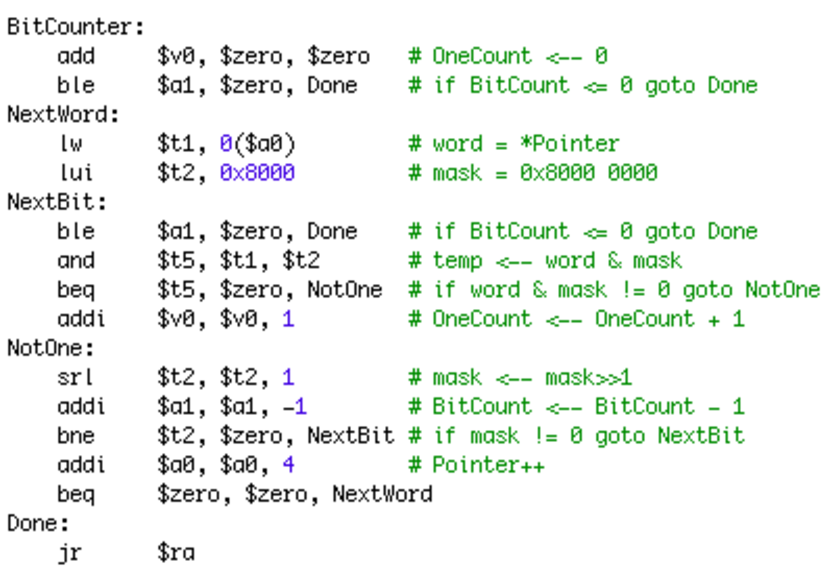
\includegraphics[width=4.0in]{BitCounterSol.pdf} 
$
\caption{\label{fig:BitCounterAlgo} MIPS Assembly Code for {\tt BitCounter}}
\end{center}
\end{figure*}
\color{black}
\else
\renewcommand{\baselinestretch}{\talllinestretch}
\begin{table}[h!] 
\centering
\begin{tabular}{c} \hline
\ \ \ \ \ \ \ \ \ \ \ \ \ \ \ \ \ \ \ \ \ \ \ \ \ \ \ \ \ \ \ \ \ \ \ \ \ \ \ \ \ \ \ \ \ \ \ \ \ \ \ \ \ \ \ \ \ \ \ \ \ \ \ \ \ \ \ \ \ \ \ \ \ \ \ \ \ \ \ \ \ \ \ \ \ \ \ \ \ \ \ \ \ \ \ \ \ \ \ \ \ \ \ \ \ \ \ \ \ \ \ \ \ \ \ \ \ \\ \hline
\\ \hline
\\ \hline
\\ \hline
\\ \hline
\\ \hline
\\ \hline
\\ \hline
\\ \hline
\\ \hline
\\ \hline
\\ \hline
\\ \hline
\\ \hline
\\ \hline
\\ \hline
\\ \hline
\\ \hline
\\ \hline
\\ \hline
\\ \hline
\\ \hline
\\ \hline
\\ \hline
\\ \hline
\\ \hline
\\ \hline
\\ \hline
\\ \hline
\end{tabular}
\end{table}
\renewcommand{\baselinestretch}{\normalstretch}
\fi

\end{question}
\end{document}


